\section{Epidemiologia e prevenzione AIDS}

\subsection{Caratteristiche e Cenni clinici}

La sindrome da immunodeficienza acquisita è stata definita come entità
nosologica nel 1981 e rappresenta lo stadio ultimo e più grave
dell'infezione da HIV, in quanto il virus colpisce e distrugge i
linfociti T e rende l'organismo incapace di difendersi da qualunque tipo
di infezione. È la conclusione di una serie di sovrainfezioni che
portano a morte.

L'AIDS è caratterizzata da:

\begin{itemize}
\item
  presenza di una o più sovrainfezioni opportunistiche
\item
  assenza di altre cause note di immunodeficienza, diverse da infezione
  da HIV
\item
  presenza di anticorpi nel sangue, poiché l'indicatore per eccellenza
  dello stato di infettività è la ricerca degli anticorpi, che vengono
  prodotti in presenza del virus (e non sono protettivi).
\end{itemize}

\emph{Caratteristiche dell'HIV:}

\begin{itemize}
\item
  Retrovirus della famiglia Lentivirus
\item
  Il nome è legato al fatto che possiede un enzima, la
  retro-trascrittasi (legata all'acido nucleico), che copia RNA a cDNA:
  questo consente al virus di inserirsi nel DNA della cellula ospite,
  integrandosi e permanendo cronicamente
\item
  La struttura è complessa, ricordiamo che:
  \begin{itemize}
  \item
    La proteina capsidica è sfruttata nell'accertamento diagnostico
  \item
    Possiede il pericapside, che lo rende fragile agli agenti naturali
    di distruzione e ai disinfettanti. Su questo si hanno:

    \begin{itemize}
    \item
      Gp41, intramembranale, che facilita l'ingresso del virus nella
      cellula ospite
    \item
      Gp120, antirecettore virale per la componente CD4, che consente
      l'aggancio alla cellula (e le cellule bersaglio principali sono i
      linfociti CD4+, per l'appunto)
    \item
      Il virus ha una duplice possibilità: lunga latenza o latenza
      seguita da malattia
    \end{itemize}
  \item
    È dotato di una grande variabilità antigenica e genotipica (si hanno
    genotipi e sotto-genotipi)
  \end{itemize}
\item
  \emph{Il processo di infezione} è composto di una serie di fasi:
  adesione alla cellula, penetrazione, scapsidamento,
  retro-trascrizione, integrazione del genoma nel DNA della cellula,
  latenza (molto lunga) e può poi iniziare la fase di replicazione che
  si conclude con la liberazione del virus, l'aggressione di altre
  cellule e la contemporanea distruzione della cellula ospite
\item
  Cellule umane sensibili ad HIV: non solo i linfociti T, ma anche altre
  cellule emopoietiche (come monociti, macrofagi), dendriti, cellule
  cerebrali, cutanee (spesso è il dermatologo il primo che sospetta l'
  infezione da HIV), gastrointestinali e altre
\item
  Ricordiamo che i linfociti T hanno un ruolo centrale per la capacità
  di difesa dell'ospite:

  \begin{itemize}
  \item
    Agiscono direttamente sui linfociti B per la produzione di anticorpi
  \item
    Inducono le cellule natural killer oltre che le T killer
  \item
    Inducono le cellule T suppressors
  \item
    Inducono la produzione di citochine per la differenziazione di altre
    cellule linfoidi
  \end{itemize}
\end{itemize}

Perciò se questi linfociti funzionano male o non ci sono viene aperta la
strada ad infezioni di qualunque tipo.

\subsection{Storia naturale della malattia}

Molto schematicamente:

\begin{itemize}

\item[1.]
  Infezione primaria (penetrazione e insediamento nella cellula)
\item[2.]
  Sieropositività: perché l'infezione si renda evidente e documentabile
  sierologicamente, vi è un periodo di latenza che va dalle 4 settimane
  ai 3 mesi (è stata osservata una positivizzazione già dopo 2
  settimane, ma in individui trasfusi con sangue infetto)
\item[3.]
  Periodo di latenza (6 mesi-13 anni, in media 8 anni; mediamente più
  breve nel bambino nato infetto)
\item[4.]
  Di qui:

  \begin{itemize}
  
  \item[a.]
    1/3 dei sieropositivi sono asintomatici o presentano linfoadenopatia
    generalizzata con sintomatologia lieve
  \item[b.]
    1/3 dei casi si manifestano infezioni AIDS correlate (A.R.C.) come
    TBC, CMV, Toxoplasmosi
  \item[c.]
    1/3 AIDS conclamato, che può insorgere anche dopo ARC
  \end{itemize}
\end{itemize}

\subsection{Accertamento diagnostico}

È uno dei pochi virus coltivabili, è stato isolato in coltura
contemporaneamente in Europa e in America. Oggi nessuno può coltivare e
lavorare HIV se non in laboratori di alta sicurezza, perciò la
diagnostica si effettua con:

\begin{itemize}
\item
  estrazione di acidi nucleici (non di routine)
\item
  ricerca di anticorpi (\emph{metodo di scelta, in quanto è
  riproducibile, standardizzabile ed economico}): le tecniche sono
  diverse, quella più utilizzata è l'immunoenzimatica (come test di
  screening) seguita poi da test di conferma. In particolare vengono
  fatti due test di screening prima di andare a dare una diagnosi così
  importante al paziente.
\end{itemize}

Poi si esegue tutta la valutazione dei parametri bioumorali, importante
del punto di vista medico (ad esempio conta dei linfociti totale e
rapporto CD4/CD8).

\subsection{Sorgente d'infezione}

\emph{Quali sono i liquidi biologici a forte rischio per contagio (cioè
in cui è stato ritrovato HIV)?}

\begin{itemize}
\item
  Sangue
\item
  Liquido seminale
\item
  Fluor vaginale
\end{itemize}

È stato riscontrato in qualche studio anche in saliva, urina, latte
umano, lacrime, ma eccezionalmente e in quantità trascurabile.

\paragraph{Modalità di trasmissione}

\begin{itemize}
\item
  Contatti sessuali (omosessuali, eterosessuali). Elementi chiave sono:

  \begin{itemize}
  \item
    Promiscuità
  \item
    Numero di partner
  \item
    Numero di rapporti sospetti
  \end{itemize}
\item
  Uso medico (non corretta conduzione dell'igiene) o rituale (in
  tossicodipendenti) di siringhe
\item
  Trasfusione di sangue (in origine era una delle cause principali di
  trasmissione, ma oggi il sangue deve essere per legge sottoposto a
  screening)
\item
  Nascita da donna infetta o malata (trasmissione verticale)
\end{itemize}

NB: un ambiente in cui il rischio di contrarre infezione è alto sono le
carceri, per l'elevato numero di fattori di rischio.

Per quanto riguarda il contagio sessuale, questo ha il massimo peso
(cioè la possibilità che il contatto si traduca in infezione) in
rapporti tra omosessuali maschi infetti, è maggiormente importante nel
rapporto tra un maschio infetto e una femmina suscettibile rispetto a
femmina infetta e maschio suscettibile (come gradualità di rischio).

\subsection{Epidemiologia}

I dati del 2015 indicano che:

\begin{itemize}
\item
  A livello mondiale, ci sono 37 milioni di soggetti infetti, di questi
  circa 2 milioni sono di età inferiore ai 15 anni.
\item
  Le nuove infezioni ogni anno sono circa 2 milioni e circa 150.000 di
  questi sono minori di 15 anni
\item
  Le morti per AIDS sono circa 1 milione e di questi circa 100.000 sono
  minori di 15 anni
\end{itemize}

La prevalenza nel mondo ha la massima intensità (2/3 dei casi) negli
Stati subsahariani dell'Africa. In Europa in particolare sono stati
registrati circa 150.000 nuove infezioni (di cui il 50\% nei Paesi
dell'est). È importante il dato dei bambini affetti da HIV, ancora oggi
significativo.

\paragraph{ASPETTI ATTUALI DELL'EPIDEMIOLOGIA}

\begin{itemize}
\item
  La trasmissione eterosessuale è fortemente incrementata, maggiore che
  nel passato, dove prevaleva la trasmissione omosessuale
\item
  Si è registrata una maggior diffusione anche al sesso femminile: il
  rapporto di incidenza tra sesso maschile e femminile all'inizio
  dell'era era 5:1, poi negli anni '90 circa 3:1 e oggi è paritario
\item
  C'è stata una diffusione dai gruppi a rischio (omosessuali,
  tossicodipendenti e trasfusioni prima degli anni '60) alla popolazione
  globale
\item
  Incremento della famacoresistenza: uso dei farmaci HIV specifici ha
  portato allo sviluppo di ceppi resistenti
\end{itemize}

\subsubsection{Epidemiologia in Italia}

Ancora oggi (dati del 2014) spicca il dato per cui \textbf{1/4 delle
persone con HIV non sa di essere infetta!} Questo anche perché il test
ha importanti limitazioni in termini di privacy. La maggior parte dei
soggetti vengono a conoscenza del proprio stato sierologico solo dopo
che si è manifestato AIDS conclamato.

Prendendo i dati epidemiologici tra 1982 e 2013:

\begin{itemize}
\item
  negli anni '90 il trend in salita della prevalenza della malattia è
  stato poi invertito grazie ad interventi terapeutici e preventivi
\item
  il maggior numero dei casi è nella popolazione italiana rispetto a
  quella straniera: le regioni più implicate sono Emilia Romagna,
  Lombardia, Toscana e Lazio
\item
  in Italia l'HIV è trasmesso più frequentemente attraverso il rapporto
  omosessuale; nella popolazione straniera invece è più importante il
  rapporto eterosessuale come modalità di trasmissione
\item
  l'età di prima diagnosi è circa intorno ai 30-40 anni (si è spostato
  in avanti di circa 10 anni rispetto al decennio scorso)
\end{itemize}

\emph{Le PATOLOGIE INDICATIVE DI AIDS più frequenti sono:}

\begin{itemize}
\item
  CMV
\item
  Sarcoma di Kaposi
\item
  Pneumocystis carinii (la prima per incidenza nel caso di trasmissione
  omosessuale ed eterosessuale)
\item
  Candidosi (che predomina insieme a Pneumocystis carinii nel caso la
  trasmissione avvenga attraverso siringhe in tossicodipendenti)
\end{itemize}

\emph{Confrontando l'epidemiologia del 2008 e del 2014:}

Nel 2008 le persone con HIV-AIDS erano 125.000-145.000, le nuove
infezioni erano 14.000 circa all'anno e nel 2014 sono 4000. La modalità
di trasmissione è rimasta uguale, attraverso rapporti sia omo- (41\%)
che etero-sessuali (43\%). L'età di infezione si è alzata da 27-29 anni
a 38-40 anni.

\subsection{Prevenzione}

\begin{itemize}
\item
  \emph{Denuncia Obbligatoria} {[}Classe III{]} con una particolare
  scheda di privacy
\item
  \emph{Accertamento Diagnostico} (visto prima)
\item
  \emph{Isolamento:} è prevalentemente per motivi terapeutici nel caso
  si tratti di situazioni critiche
\item
  \emph{Disinfezione:} è un virus relativamente fragile, infatti sono
  molti i principi attivi efficaci su HIV:

  \begin{itemize}
  \item
    H2O2 a concentrazioni maggiori del 6\%: distrugge il virus in 30'
  \item
    Ipocloriti anche a concentrazioni non molto elevate (0,1-0,5\%) in
    20'
  \item
    Glutaraldeide al 2\% in 30'
  \item
    Iodofori a concentrazione discreta
  \item
    Autoclave: funziona molto bene (121\textsuperscript{o} in 15-30')
  \item
    Gas plasma per strumenti più delicati
  \end{itemize}

\begin{quote}
NB: è un virus molto fragile nell'ambiente, anche a livello domestico lo
possiamo abbattere facilmente: non resiste al calore (è sufficiente la
lavatrice a 60\textsuperscript{o} e se si aggiungono per esempio dei prodotti a base di
cloro c'è la certezza di disinfettare in modo adeguato)
\end{quote}

\item
  \emph{Importanti l'educazione sanitaria e le norme comportamentali,}
  date le modalità di trasmissione
\item
  \emph{Profilassi mirata:} può essere

  \begin{itemize}
  \item
    PRIMARIA: ha lo scopo di evitare l'infezione
  \item
    SECONDARIA: ha lo scopo di evitare che ci sia il passaggio da
    infezione da HIV ad AIDS
  \end{itemize}
\end{itemize}

\subsubsection{Prevenzione Mirata Primaria}

La prevenzione mirata primaria si
avvale di due mezzi:

\begin{itemize}

\item[1.]
  ATTI IMPOSITIVI (ciò che la legge impone che venga fatto):

  \begin{itemize}
  \item[a.]
    Segnalazione dei casi
  \item[b.]
    Controllo del sangue e degli emoderivati ad uso umano (legge del
    1985; ricordiamo nel 1971 quella per HBV e nel 1989 quella per HCV)
  \end{itemize}
  
\item[2.]
  SUGGERIMENTI COMPORTAMENTALI: informazione e formazione sui
  comportamenti a rischio:

  \begin{itemize}
 
  \item[a.]
    Rapporti tra omosessuali: utilizzo dei mezzi di prevenzione
  \item[b.]
    Tossicodipendenti: non scambiare le siringhe
  \item[c.]
    Neonati: educazione alla salute del sesso femminile per quanto
    riguarda i proprio rischi (droga e partner sessuale)
  \item[d.]
    Popolazione generale: conoscenza del rischio legato alla promiscuità
    sessuale e la possibilità di precauzione
  \item[e.]
    Mondo sanitario: evitare di pungersi con strumenti utilizzati sui
    pz, mettere in atto le \textbf{precauzioni standard e/o universali}
    di disinfezione: \emph{applicare i mezzi di barriera per evitare il
    contatto parenterale, cutaneo, mucoso di sangue o altri liquidi
    biologici; lavaggio delle mani nei 5 momenti; utilizzo di guanti,
    camici, occhiali o visiere; attenzione nella raccolta e al
    processamento di materiali contaminati (pulizia, decontaminazione e
    sterilizzazione); smaltimento dei rifiuti in modo adeguato.}
  \end{itemize}
\item[3.]
  Non esiste ad oggi un vaccino specifico (ma ci sono studi piuttosto
  avanzati in merito)
\end{itemize}

\emph{Rischio di infezione in ambito sanitario a seconda del tipo di
esposizione e del pz fonte:}

\begin{itemize}
\item
  Ferite profonde e sanguinanti, così come la puntura con ago cavo da
  prelievo, sono al primo livello di rischio (vedi tabella*)
\item
  Presenza di sangue in quantità significativa su superfici e presidi
  medici
\item
  Contaminazione congiuntivale massiva
\item
  Le caratteristiche del paziente fonte che aumentano il rischio sono:

  \begin{itemize}
  \item
    Pz con \textgreater{}30.000 copie di RNA per ml di sangue
  \item
    pz in fase terminale
  \item
    pz con infezione acuta
  \item
    pz con sospetta resistenza ai farmaci antivirali
  \end{itemize}
\end{itemize}

* è stato fatto uno studio che mette in luce il rischio di infezione in
seguito a puntura con ago cavo da prelievo, in pz affetti da HBV, HCV,
HIV: il rischio più significativo è per HBV, poiché è molto concentrato
nel sangue per esempio, inoltre è molto resistente nell'ambiente.

\begin{figure}[!ht]
\centering
	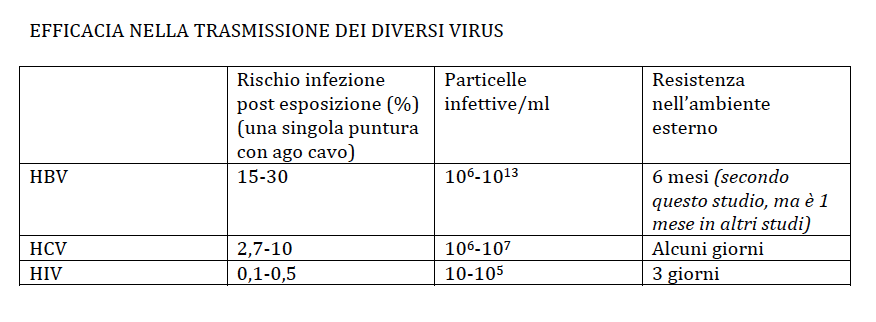
\includegraphics[width=0.3\textwidth]{12/image1.png}
	\end{figure}

\subsubsection{Prevenzione Mirata Secondaria}

Ha lo scopo di prevenire il passaggio da sieropositivo ad AIDS (o a
patologie correlate ad AIDS) e si avvale di:

\begin{itemize}
\item[1.]
  \emph{potenziamento delle condizioni fisiche}: tenere il fisico in
  condizioni ottimali
\item[2.]
  \emph{aiutare con la somministrazione di immunomodulatori}
\item[3.]
  \emph{diagnosi precoce:} conoscenza della sieropositività e
  trattamento precoce delle infezioni opportunistiche
\item[4.]
  \emph{chemioprofilassi}: utilizzare farmaci per HIV su un soggetto
  sieropositivo (e non ha AIDS) è un'azione di profilassi secondaria; si
  parla propriamente di terapia se questi farmaci vengono utilizzati su
  soggetto con AIDS: lo stesso farmaco può essere utilizzato per tener
  bassa la viremia ed evitare AIDS, oppure per ridurre viremia in
  soggetto con AIDS.
\end{itemize}

\subsubsection{Farmaci per HIV}

I principali farmaci sono:

\begin{itemize}
\item
  inibitori nucleosidici della retrotrascrittasi
\item
  inibitori non nucleosidici della retrotrascrittasi
\item
  inibitosi della proteasi
\end{itemize}

e il loro utilizzo combinato nella triplice terapia fa sì che si riduca
la farmaco resistenza, dato che hanno bersagli diversi. La letalità per
AIDS si è fortemente ridotta grazie al trattamento profilattico e
chemioterapeutico.

\subsection{Prevenzione vaccinale}

Sono molteplici i gruppi di studio per la creazione di un vaccino
specifico, ma gli ostacoli alla creazione di un vaccino specifico sono:

\begin{itemize}
\item[1.]
  Il virus che ha la capacità di sfuggire al controllo del sistema
  immunitario (è un virus intracellulare integrato)
\item[2.]
  ha capacità di distruggere le cellule immunocompetenti
\item[3.]
  ha una lunga latenza
\item[4.]
  estrema variabilità antigenica
\item[5.]
  non esiste un reale modello animale con una patologia che ricalchi
  l'infezione da HIV dell'uomo
\end{itemize}

Sono stati fatti tantissimi tentativi di approccio ad un possibile
vaccino, il più interessante (\emph{è un progetto italiano}) è il
vaccino contro la \emph{proteina Tat}: è una proteina regolatoria di
HIV, necessaria per la replicazione completa del virus e prodotta dopo
che il virus è entrato nella cellula. Il razionale della scelta di
azione verso questa proteina è motivato dal fatto che gli anticorpi anti
Tat sembrano:

\begin{itemize}
\item[1.]
  rallentare la malattia
\item[2.]
  sono più frequenti nello stadio asintomatico rispetto agli stadi più
  avanzati
\item[3.]
  i linfociti T citotossici anti-Tat sono presenti nell'individuo
  sieropositivo e agiscono distruggendo le cellule infettate da HIV
\item[4.]
  le regioni immunogeniche della Tat sono uguali nei diversi ceppi
  virali
\end{itemize}

Gli studi sperimentali sul modello animale hanno dimostrato che questo
vaccino non ha effetti tossici, è in grado di indurre un'immunità sia
umorale che cellulare, agendo sull'attività replicativa del virus. Se
gli studi avranno successo questo sarà un \textbf{vaccino di tipo
terapeutico}, da dare ad un soggetto sieropositivo per controllare
l'attività replicativa del virus. Nel 2003 era partita la prima fase, è
già partita la seconda fase e ci sono studi di fase avanzata in
popolazioni ad alto rischio.

\section{Epatite A (HAV)}

\subsection{Caratteristiche e Cenni clinici}

Il virus dell'epatite A è un virus a \textbf{trasmissione fecale orale:}
a questo circuito di trasmissione appartengono in particolare HAV, HEV,
Poliovirus e Febbre Tifoide. HEV nella nostra epidemiologia, e in quella
degli altri Paesi industrializzati, è un nuovo problema in crescita,
soprattutto come virus da importazione. La trasmissione fecale è di tipo
indiretto, attraverso le feci (e le urine contaminate, in particolare
nella febbre tifoide) e l'assunzione di alimenti e acqua contaminata, ma
si ha anche una trasmissione diretta per via personale (per cattiva
igiene). Importantissimi nel circuito di trasmissione fecale orale sono
i vettori (mosche), la contaminazione degli ambienti, degli alimenti e
delle acque. Sono agenti che resistono discretamente nell'ambiente.

HAV è un piccolo virus ad RNA (hepa-RNA virus), di struttura
eicosaedrica e nudo, privo di pericapside (quindi più resistente).
Caratteristiche:

\begin{itemize}
\item
  È presente un unico sierotipo
\item
  È specie specifico
\item
  Può dare origine ad una infezione asintomatica (più frequente) o ad
  una infezione acuta conclamata
\item
  Non c'è MAI la CRONICIZZAZIONE
\item
  All'infezione segue la formazione di anticorpi con immunità duratura
  per tutta la vita
\item
  Ha una discreta resistenza agli agenti fisici e chimici: calore (56\textsuperscript{o}
  per 30'), etere, ph 3 (e infatti passa la barriera gastrica), permane
  per giorni e/o settimane nei mitili, nell'acqua, nel suolo, nel
  sedimento marino
\item
  È un virus coltivabile, ma per la \emph{diagnosi} si fa la ricerca con
  il microscopio elettronico o si utilizza la biologia molecolare. Il
  materiale di scelta sono le feci.
\end{itemize}

\subsection{Storia naturale della malattia}

Su 10.000 contagiati nel 90\% dei casi si ha forma subclinica,
anitterica. Solo nel 10\% dei casi si ha epatite acuta e tra questi nel
10\% dei casi la malattia è fulminante. NON C'È MAI CRONICITÀ.

La massima infettività documentata è da due settimane prima dell'esordio
fino a 2 settimane dopo l'insorgenza dell'ittero. Teniamo presente che
il virus diffonde attraverso il sangue, quindi è possibile una
trasmissione per via ematica, ma è molto rara. La via principale di
trasmissione è quella fecale-orale.

\emph{Il periodo di incubazione medio è di 30 giorni}: può andare da 7 a
50 giorni. La forma sintomatica è più presente nel bambino che
nell'adulto.

\emph{Vediamo l'andamento sierologico:}

\begin{figure}[!ht]
\centering
	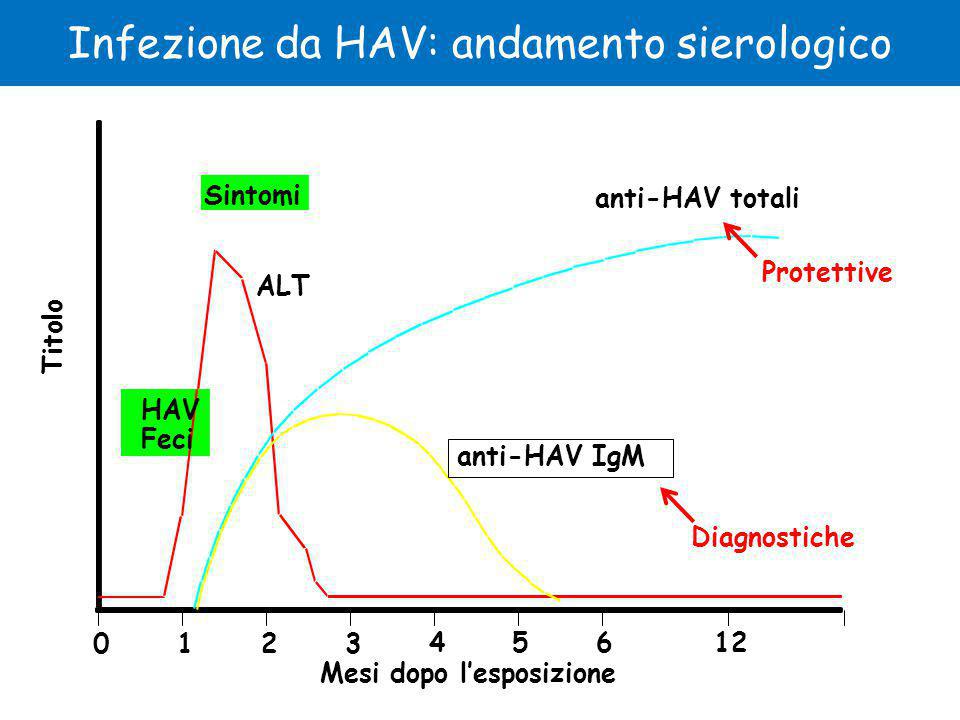
\includegraphics[width=0.3\textwidth]{12/image2.png}
	\end{figure}

\begin{itemize}
\item
  Il virus è presente nelle feci già prima della comparsa dei segni
  clinici
\item
  Si ha il movimento degli enzimi epatici: sofferenza epatica
\item
  Quando virus comincia ad esaurirsi nelle feci e la viremia si riduce
  si ha la concomitante comparsa di anticorpi protettivi nel sangue
\end{itemize}

\subsection{Vie di trasmissione}

\emph{La trasmissione del virus dell'epatite A:}

\begin{itemize}
\item
  è principalmente attraverso il circuito fecale-orale: le feci
  contengono una concentrazione di 10\textsuperscript{10} virus per ml:
  si considerino non solo gli alimenti e le acque contaminate, ma anche
  le acque per la balneazione!
\item
  il contagio interumano è importante (cattiva igiene)
\item
  si può trasmettere per via indiretta attraverso vettori (mosche) e
  veicoli (acqua e alimenti)
\item
  esposizione a sangue contaminato (nella fase di diffusione per via
  ematica la concentrazione del virus è circa 10\textsuperscript{4}):
  problema molto contenuto
\end{itemize}

\subsection{Epidemiologia}


HAV è presente in tutto il mondo, particolarmente in Paesi in condizioni
igienico sanitarie scadenti, tanto che l'incidenza di HAV è un
indicatore delle condizioni di sviluppo.

La forma silente può essere cercata con la ricerca degli anticorpi nella
popolazione:

\begin{itemize}
\item
  98\% in India
\item
  10\% in USA
\item
  5\% in Svizzera
\end{itemize}

\emph{Secondo l'OMS la prevalenza è di circa 1,5 milioni di casi clinici
(sintomatici) ogni anno, nel mondo.}

Dal punto di vista dell'andamento dell'infezione, questo è generalmente
sporadica, ma vi possono essere epidemie nelle comunità a rischio, come
quelle infantili o i collegi, per le condizioni igieniche più favorevoli
alla diffusione, l'affollamento, le abitudini alimentari. Gli ultimi
dati europei vedono un trend in salita della malattia e la distribuzione
per età vede come massimo peso i bambini e gli anziani.

Riassumendo i fattori di rischio sono:

\begin{itemize}
\item
  persone a contatto con soggetti infetti
\item
  bambini in comunità chiuse
\item
  viaggiatori in aree endemiche
\item
  tossicodipendenti
\end{itemize}

NB: Ci sono zone ad alta, moderata, bassa e molto bassa endemia, legate
alla prevalenza dei diversi fattori di rischio (per esempio nelle zone a
molto bassa endemia, la presenza di questo virus è essenzialmente legata
ai viaggiatori).

\subsubsection{Epidemiologia in Italia}


\begin{itemize}
\item
  La siero-epidemiologia della popolazione italiana vede una
  distribuzione del virus con prevalenza al sud, con incremento della
  positività agli anticorpi con il crescere dell'età: dopo i 40 anni più
  del 50\% della popolazione ha gli anticorpi (senza storia di malattia
  evidente).
\item
  Importanti nella nostra realtà epidemiologica sono i viaggiatori: si
  stima che la prevalenza sia da 30 a 300 casi per 10.000 viaggiatori in
  un mese di viaggio.
\item
  La principale sorgente di infezione è il portatore sano, così come il
  portatore precoce. Non abbiamo mai il portatore cronico.
\item
  La principale \emph{età} nella quale si va incontro all'infezione è
  quella giovanile: 15-24 anni
\item
  Tra tutte le epatiti, HAV prevale in assoluto, con forti epidemie nel
  1997 e nel 2007, ma anche piccoli e medi focolai epidemici nel 2001,
  2004, 2009 e 2013, collocati principalmente al sud.
\end{itemize}

\begin{figure}[!ht]
\centering
	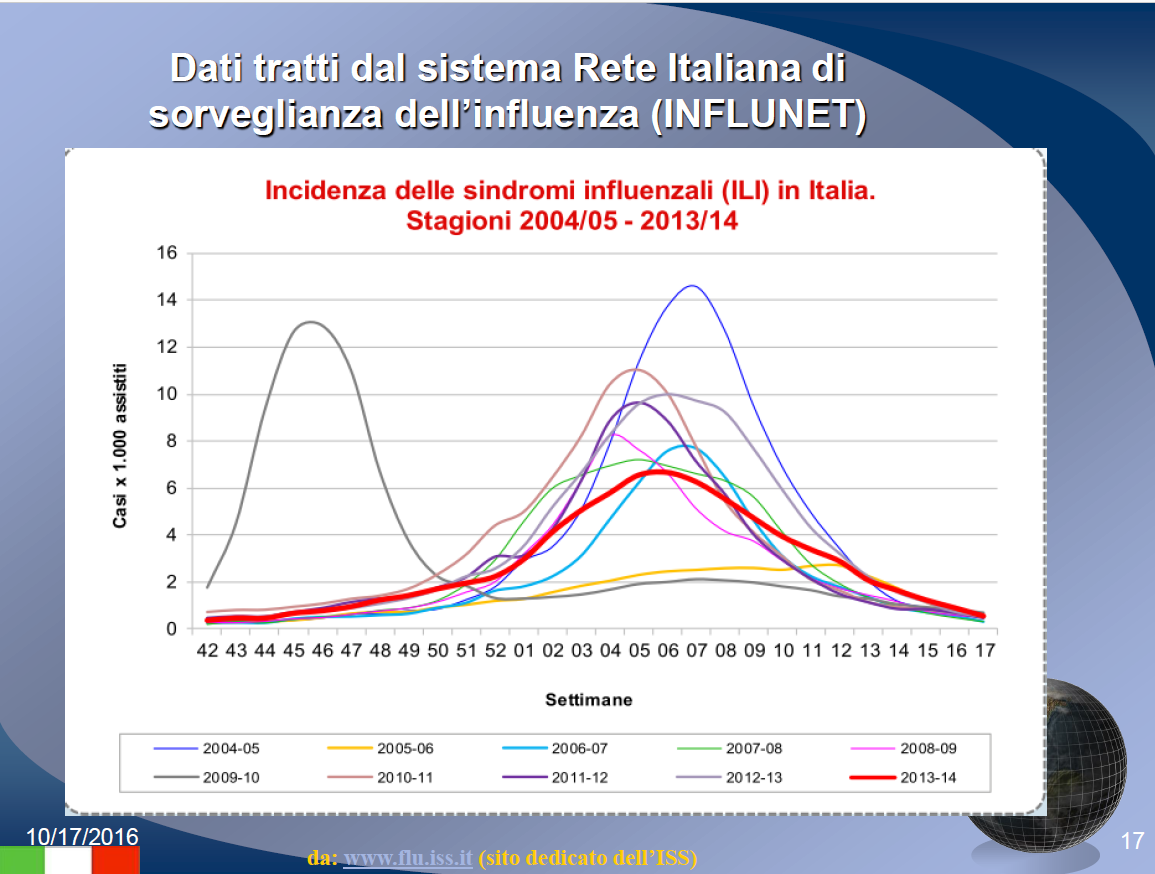
\includegraphics[width=0.7\textwidth]{02/image3.png}
\end{figure}


\begin{itemize}
\item
  FATTORI DI RISCHIO DOCUMENTATI IN ITALIA:

  \begin{itemize}
  \item
    Viaggio all'estero (è il più importante)
  \item
    Per l'alimentazione: il consumo di militii, soprattutto in certe
    regioni e in certi periodi dell'anno
  \item
    Contatti di familiari infetti
  \end{itemize}
\end{itemize}
\subsection{Prevenzione}


\begin{enumerate}
\def\labelenumi{\arabic{enumi}.}
\item
  INDIRETTA: è un aspetto di tipo generale, ha una valenza molteplice e
  in questo caso vale per TUTTI gli agenti del circuito fecale-orale, in
  linea di massima. È rivolta sia all'ambiente che alla persona.

  \begin{enumerate}
  \def\labelenumii{\alph{enumii}.}
  \item
    CONTROLLO DELLA MATRICE AMBIENTALE

    \begin{enumerate}
    \def\labelenumiii{\roman{enumiii}.}
    \item
      Alimenti: controllo della produzione e vendita, soprattutto dei
      frutti di mare, che assumono nutrienti attraverso la filtrazione
      dell'acqua in cui vivono, perciò la concentrazione dei patogeni
      all'interno di questi è molto più concentrata (in termini
      logaritmici) rispetto alle acque in cui si trovano.
    \item
      Acqua: controllo di acqua, perché sia igienicamente sicura, e
      offrire a tutta la popolazione l'acqua potabile
    \item
      Controllo del trattamento e dello smaltimento dei liquami fognari
    \item
      Lotta ai vettori (mosche) con disinfestazione
    \end{enumerate}
  \item
    EDUCAZIONE SANITARIA (in realtà è una via di mezzo tra prevenzione
    indiretta e diretta): consiste nell'importanza del rispetto delle
    norme igieniche per coloro che:

    \begin{enumerate}
    \def\labelenumiii{\roman{enumiii}.}
    \item
      Manipolano o servono alimenti
    \item
      Sono addetti all'assistenza di bambini o di malati
    \end{enumerate}
  \end{enumerate}
\item
  DIRETTA: mirata al virus


\begin{itemize}
\item
   
  \emph{Denuncia Obbligatoria} {[}Classe II{]}
   
\item
   
  \emph{Isolamento:} non obbligatorio, ma importante dal punto di vista
  dell'igiene, per contenere l'infezione nell'ambiente del malato
   
\item
   
  \emph{Inchiesta epidemiologica,} per capire perché si sia manifestata
  la patologia ed individuare la sorgente e il veicolo di infezione
   
\item
   
  \emph{Disinfezione continua e terminale} (il virus è discretamente
  resistente in ambiente e in acqua)
   
\item
   
  \emph{Profilassi Immunitaria Specifica:} esiste un vaccino per HAV.
   
\end{itemize}
\end{enumerate}
\subsubsection{Immunoprofilassi attiva: il Vaccino per HAV}


Il vaccino è stato ottenuto con virus ucciso, coltivato su cellule
diploidi umane e inattivato con formolo, da somministrare per via
intramuscolare profonda (come tutti i vaccini con patogeni inattivati).
Le dosi per una completa vaccinazione sono a 0-1-6 mesi e l'efficacia è
molto elevata: nel 90\% dei vaccinati è documentabile la presenza di IgG
dopo la prima dose e la totalità nella seconda dose con anticorpi
duraturi. La terza dose ha proprio la funzione di aumentare in titolo
anticorpale e l'efficacia del vaccino nel tempo che si attesta intorno
ai 20 anni.
\\\\
\emph{Effetti collaterali del vaccino:} dolorabilità, cefalea e
malessere di breve durata.

\paragraph{Strategia vaccinale}


\begin{itemize}
\item
  \emph{Pre-esposizione:} è consigliato il vaccino:

  \begin{itemize}
  \item
    In primis ai viaggiatori in aree endemiche, almeno due dosi o dosi
    doppie se il tempo prima del viaggio è breve
  \item
    Ai soggetti che vivono in zone ad alta endemia
  \item
    A soggetti che sono a rischio di contatto in ambito lavorativo
    (operatori sanitari e addetti allo smaltimento dei rifiuti)
  \item
    Ai militari che prestano servizio in aree endemiche
  \item
    Soggetti con handicap istituzionalizzati (per incapacità fisica o
    mentale di mettere in atto le norme igieniche)
  \item
    Soggetti con malattie croniche
  \item
    Tossicodipendenti
  \end{itemize}
\item
  \emph{Post-esposizione:} c'è la possibilità di applicare il vaccino
  post-esposizione: anche se oggi non si hanno ancora dati scientifici
  certi, data l'elevata quantità di anticorpi prodotti dopo una sola
  somministrazione, si può utilizzare questa modalità in un focolaio
  epidemico, proprio all'inizio dell'epidemia, per contenere il
  contagio.
\end{itemize}

\subsubsection{Immunoprofilassi Passiva}



In caso di probabile contagio è possibile usare le immunoglobuline
specifiche, che potrebbero essere previste anche come somministrazione
pre esposizione per i viaggiatori in aree a media ed alta endemia, e
soprattutto post esposizione per contatti a rischio.


\section{Epatite E (HEV)}



\subsection{Caratteristiche e Cenni clinici }


Il virus dell'epatite E è stato scoperto in un focolaio endemico in
India. È trasmesso attraverso un circuito fecale-orale e ha periodo di
incubazione simile all'HAV, di circa 40 giorni (range dai 15 ai 60
giorni).

Ha una notevole importanza nelle donne in gravidanza dove l'infezione si
associa ad una letalità del 15-25\% dei casi, contro la letalità nella
popolazione generale dell'1-3\%. La gravità della malattia aumenta con
il crescere dell'età, ma il virus NON determina MAI CRONICIZZAZIONE.

\emph{La diagnosi si avvale di:}

\begin{itemize}
\item
  Clinica
\item
  Anticorpi specifici
\item
  Ricerca di acidi nucleici (attraverso RT-PCR) in campioni di sangue e
  feci
\end{itemize}

\subsection{Epidemiologia e Profilassi}


\emph{La distribuzione del mondo}: HEV è prevalente nel subcontinente
indiano, dove è stato identificato, ed è più presente in Paesi in via di
sviluppo che nei Paesi industrializzati. Secondo la WHO nel 2014 si sono
registrati circa \emph{20 milioni di casi a livello mondiale.}

Si sono verificati dei focolai epidemici, quasi sempre associati
all'acqua contaminata da liquami fognari; è rarissimo il contagio
interumano. Negli USA, dove ci sono più dati, l'infezione da HEV è
generalmente associata a viaggi in zone endemiche. In \emph{Italia} è
rara, ma si sono registrati negli ultimi anni dei focolai epidemici
nelle regioni centrali.
\subsection{Prevenzione}


Si possono solo attuare solamente delle azioni di \emph{prevenzione
generale} per coloro che si recano in Paesi endemici, per esempio:

\begin{itemize}
\item
  Utilizzare sempre e solo acqua potabile (in contenitori tappati)
\item
  Non bere bibite con ghiaccio
\item
  Consumare frutti di mare cotti (la cottura abbatte il virus)
\item
  Consumare verdure preferibilmente cotte e la frutta è da sbucciare
  dopo il lavaggio
\end{itemize}

Non abbiamo dati su eventuale immunoprofilassi con IgG e non abbiamo un
vaccino globalmente accettato, anche se nel 2011 in Cina è stato
licenziato un vaccino specifico.
\section{Febbre Tifoide}

\subsection{Caratteristiche e Cenni clinici}


Malattia infettiva determinata da Salmonella Typhi, che appartiene alla
famiglia delle salmonelle ed è dotata di alcuni \emph{antigeni:}

\begin{itemize}
\item
  Antigene O: somatico
\item
  Antigene H: flagellare
\item
  Antigene Vi: capsulare
\end{itemize}

Ed è proprio verso questi antigeni che vengono prodotti gli anticorpi
protettivi, il più importante è quello verso l'antigene capsulare,
l'anticorpo anti-Vi, insieme anche all'anti-O.

La febbre tifoide è una malattia molto meno frequente che nel passato;
al giorno d'oggi, in assenza di terapia, presenta una letalità che va
dall'1 al 10\% a seconda delle aree.

Il problema attuale è la crescente farmaco resistenza, molto più
presente nei Paesi del terzo mondo, in particolare in alcune regioni del
sud est asiatico (dove si calcola che il 70\% dei ceppi isolati presenta
una farmaco resistenza).

\subsection{Storia naturale della malattia }

Trasmesso per via fecale orale, è in grado di superare la barriera
gastrica e ciò avviene più facilmente se:

\begin{itemize}
\item
  è presente in carica virale molto elevata
\item
  si consuma un pasto ricco di proteine (che hanno un'azione
  neutralizzante l'acidità gastrica)
\item
  si beve acqua in quantità abbondante (diluizione)
\item
  si ha una condizione di ipocloridia gastrica
\end{itemize}

da qui, dopo una prima fase di replicazione (in era pre antibiotica) il
batterio passa alle strutture linfatiche della parete intestinale -> dotto
toracico -> diffusione ematica -> diffusione ai linfonodi -> dal fegato
attraverso la bile torna una seconda volta a livello intestinale, dove
si realizza la seconda replicazione, con la moltiplicazione in strutture
già sensibilizzate: questo innesca un grosso processo flogistico con
escare e necrosi, ulcerazioni, fino ad avere lesioni vascolari,
emorragie e quindi la morte del paziente.

L'accertamento diagnostico permette di individuare:

\begin{itemize}
\item
  nella prima settimana, la presenza del patogeno nel sangue, attraverso
  emocoltura
\item
  nella seconda settimana anticorpi anti-O e anti-H con
  sieroagglutinazione
\item
  nella terza e quarta settimana la ricerca del patogeno nella
  coprocoltura. Il patogeno può essere abbondantemente presente anche
  nelle urine.
\end{itemize}

\subsection{Epidemiologia e Profilassi}


L'infezione si registra prevalentemente nei Paesi sottosviluppati,
Indonesia, Guinea, Haiti, che oltre ad essere paesi dal clima caldo
presentano condizioni igienico-sanitarie scadenti.

\emph{In Europa} la prevalenza è calata notevolmente nell'ultimo
decennio, ma rimane ancora discreta la prevalenza negli stati dell'est.

\emph{In Italia} l'incidenza si attesta intorno a 1/100.000 casi
all'anno, con prevalenza maggiore al sud e nelle isole, dove abitudini
alimentari, condizioni igieniche, ma anche cultura alimentare (consumo
di frutti di mare crudi) favoriscono la diffusione della malattia.

\subsection{Sorgente d'infezione}


È un'infezione esclusivamente umana (diversamente dalle altre
salmonelle) e le principali sorgenti di infezione sono il malato, ma
anche il portatore convalescente e il portatore cronico.

La \emph{trasmissione è per via fecale orale}: possiamo rifarci a ciò
che era stato detto a riguardo nel HAV.

Si noti che nel nord-Italia si registrano dei casi nel periodo post
Natale in soggetti che durante le vacanze si recano nei paesi di
origine, acquisiscono le abitudini alimentari, tornano in Italia e
manifestano la malattia. È un'infezione molto più frequente nel bambino
e nel giovane adulto.

\subsection{Prevenzione}


Per la \emph{profilassi indiretta}: vale esattamente il discorso fatto
per HAV, con il controllo delle matrici ambientali e l'educazione alla
salute (che valgono per tutte le patologie del circuito fecale-orale).
\\\\
La \emph{profilassi diretta}:

\begin{itemize}
\item
   
  \emph{Denuncia Obbligatoria} {[}Classe II{]}
   
\item
   
  \emph{Isolamento:} non obbligatorio, ma è importante dal punto di
  vista dell'igiene, per contenere l'infezione nell'ambiente del malato.
  Tre campioni di feci devono risultare negativi dopo l'inizio del
  trattamento antibiotico per considerare il soggetto non più
  infettante.
   
\item
   
  \emph{Accertamento diagnostico:} importante perché c'è la figura del
  portatore cronico
   
\item
   
  \emph{Inchiesta epidemiologica,} per capire perché si sia manifestata
  la patologia ed individuare la sorgente e il veicolo di infezione
   
\item
   
  \emph{Disinfezione continua} (le feci sono contaminate per lungo
  tempo) \emph{e terminale e disinfestazione} (mosche)
   
\item
   
  \emph{Profilassi Immunitaria Specifica:} esiste un vaccino specifico
  per S. typhi.
   
\end{itemize}

\subsubsection{Immunoprofilassi Attiva}


È stata una delle patologie più studiate e quello verso la Salmomella
Typhi è stato il vaccino più precocemente ricercato nella storia, tanto
che sono state tentate tantissime strade per la sua realizzazione.

Ad oggi disponiamo di 3 vaccini:

\begin{itemize}
\item
  Il vecchio vaccino, ancora utilizzato, somministrato per via
  parenterale
\item
  Vaccino Ty21: vivo ed attenuato ad uso naturale, viene somministrato
  per via orale segue la via dell'infezione naturale.

  \begin{itemize}
  \item
    È stato ottenuto privando il batterio virulento di un enzima, che
    rende il batterio incapace di incorporare galattosio nel LPS della
    parete cellulare. Il ceppo si sviluppa come variante rugosa non
    patogena, inizialmente non immunizzante, ma quando giunge in un
    ambiente ricco di galattosio (come l'intestino), questo zucchero
    viene assunto dall'ambiente, utilizzato per la costruzione della
    parete cellulare e il patogeno riesce a fare una serie di cicli
    replicativi (il batterio diventa così immunizzante), ma non riesce
    ad eliminare il galattosio accumulato, quindi esso si autolisa
    proprio per l'eccesso osmotico: questa salmonella non viene dunque
    eliminata con le feci e il patogeno è divenuto sì immunizzante
    nell'intestino, ma non esce come virulento, grazie al processo di
    autolisi: perciò non è diffuso nell'ambiente
  \item
    È molto immunizzante (efficacia maggiore dell'87\% per più di 3
    anni)
  \item
    Viene assunto in capsule gastroresistenti un'ora prima del pasto per
    3 giorni, a giorni alterni, e si può ripetere per mantenere
    l'immunità elevata per tempi lunghi
  \item
    Non abbiamo dati per un'eventuale utilizzo post esposizione del
    vaccino
  \item
    NB: essendo un vaccino con ceppo vivo non possiamo somministrarlo in
    concomitanza con la terapia antibiotica
  \end{itemize}
\item
  \emph{Vaccino a componente Vi:} somministrato per via parenterale, ha
  efficacia circa uguale al vaccino Ty21, con durata di circa 3 anni. È
  ben tollerabile.
\end{itemize}

\paragraph{Indicazioni per la vaccinazione:}


\begin{itemize}
\item
  In primis c'è una forte indicazione (ma non l'obbligo) per chi si reca
  in aree endemiche
\item
  A chi svolge attività a rischio, come pulizia di ospedali, personale
  addetto al trasporto di malati
\item
  Agli operatori sanitari
\item
  Al personale addetto all'approvvigionamento idrico e alla
  manipolazione del latte
\item
  Al personale addetto alla raccolta e allo smaltimento dei rifiuti
\item
  A chi svolge manipolazione e vendita di alimenti: in passato il
  vaccino era d'obbligo (DPR n 327/1980), ma oggi l'igiene degli
  ambienti è regolata dalle regioni, che hanno sostituito il libretto
  sanitario con controlli degli ambienti e corsi di formazione tenuti
  dalle AUSL
\end{itemize}

